% !TEX encoding = UTF-8 Unicode
% !TEX root = thesis-ex.tex

This section will discuss the momentum profile of the jet as measured by the CMS detector for \pbpb\ collisions at $\sqrtsnn = 5.02$ TeV \cite{Sirunyan:2018jqr}.
This can be considered to be an extension to a fragmentation function measurement in that it provides information about the momentum distribution of charged particles not only within the jet boundary, but also outside.
The jet profile is defined as the distribution of particle yields in an annulus of width $\Delta r$ and is given as:
\begin{align}
%\rho(\Delta r) = \frac{1}{\sum_{\rm jets} \sum_{\rm tracks} \pTtrk} \left[ \frac{1}{\delta r} \frac{1}{\Njet} \sum\nolimits_{\rm jets}  \sum\nolimits_{{\rm tracks} \in (\Delta r_a, \Delta r_b)} \pTtrk   \right]
P(\Delta r) = \frac{1}{\delta r} \frac{1}{\Njet} \sum\nolimits_{\rm jets}  \sum\nolimits_{{\rm tracks} \in (\Delta r_a, \Delta r_b)} \pTtrk   
\end{align}
where $\Delta r_a$ and $\Delta r_b$ are the edges of the annulus at $\Delta R$, and $\delta r = \Delta r_b - \Delta r_a$.

The jet profile for \pp, \pbpb, and the modification to the jet shape variable are shown in Figure~\ref{fig:jetshape_cms}.
It can be seen from the bottom panels of Figure~\ref{fig:jetshape_cms} that there is an excess of low \pt\ particles in \pbpb\ compared to \pp\ at intermediate and large distances from the jet axis.
This enhancement is compensated by a depletion of high \pt\ particles ($\pt > 4$ GeV) at all angles.
In particular, the depletion in particle yields in 0--10\% central \pbpb\ is up to almost half the particle yields in \pp\ for $\Delta r > 0.4$.
The modifications be described in terms of jet quenching, coupled with effects from the wake the jet as it propagates through the QGP.
This wake can cause an enhancement in the low \pt\ yield of particles that is most easily seen at large angles.

\begin{figure}[htbp]
\begin{center}
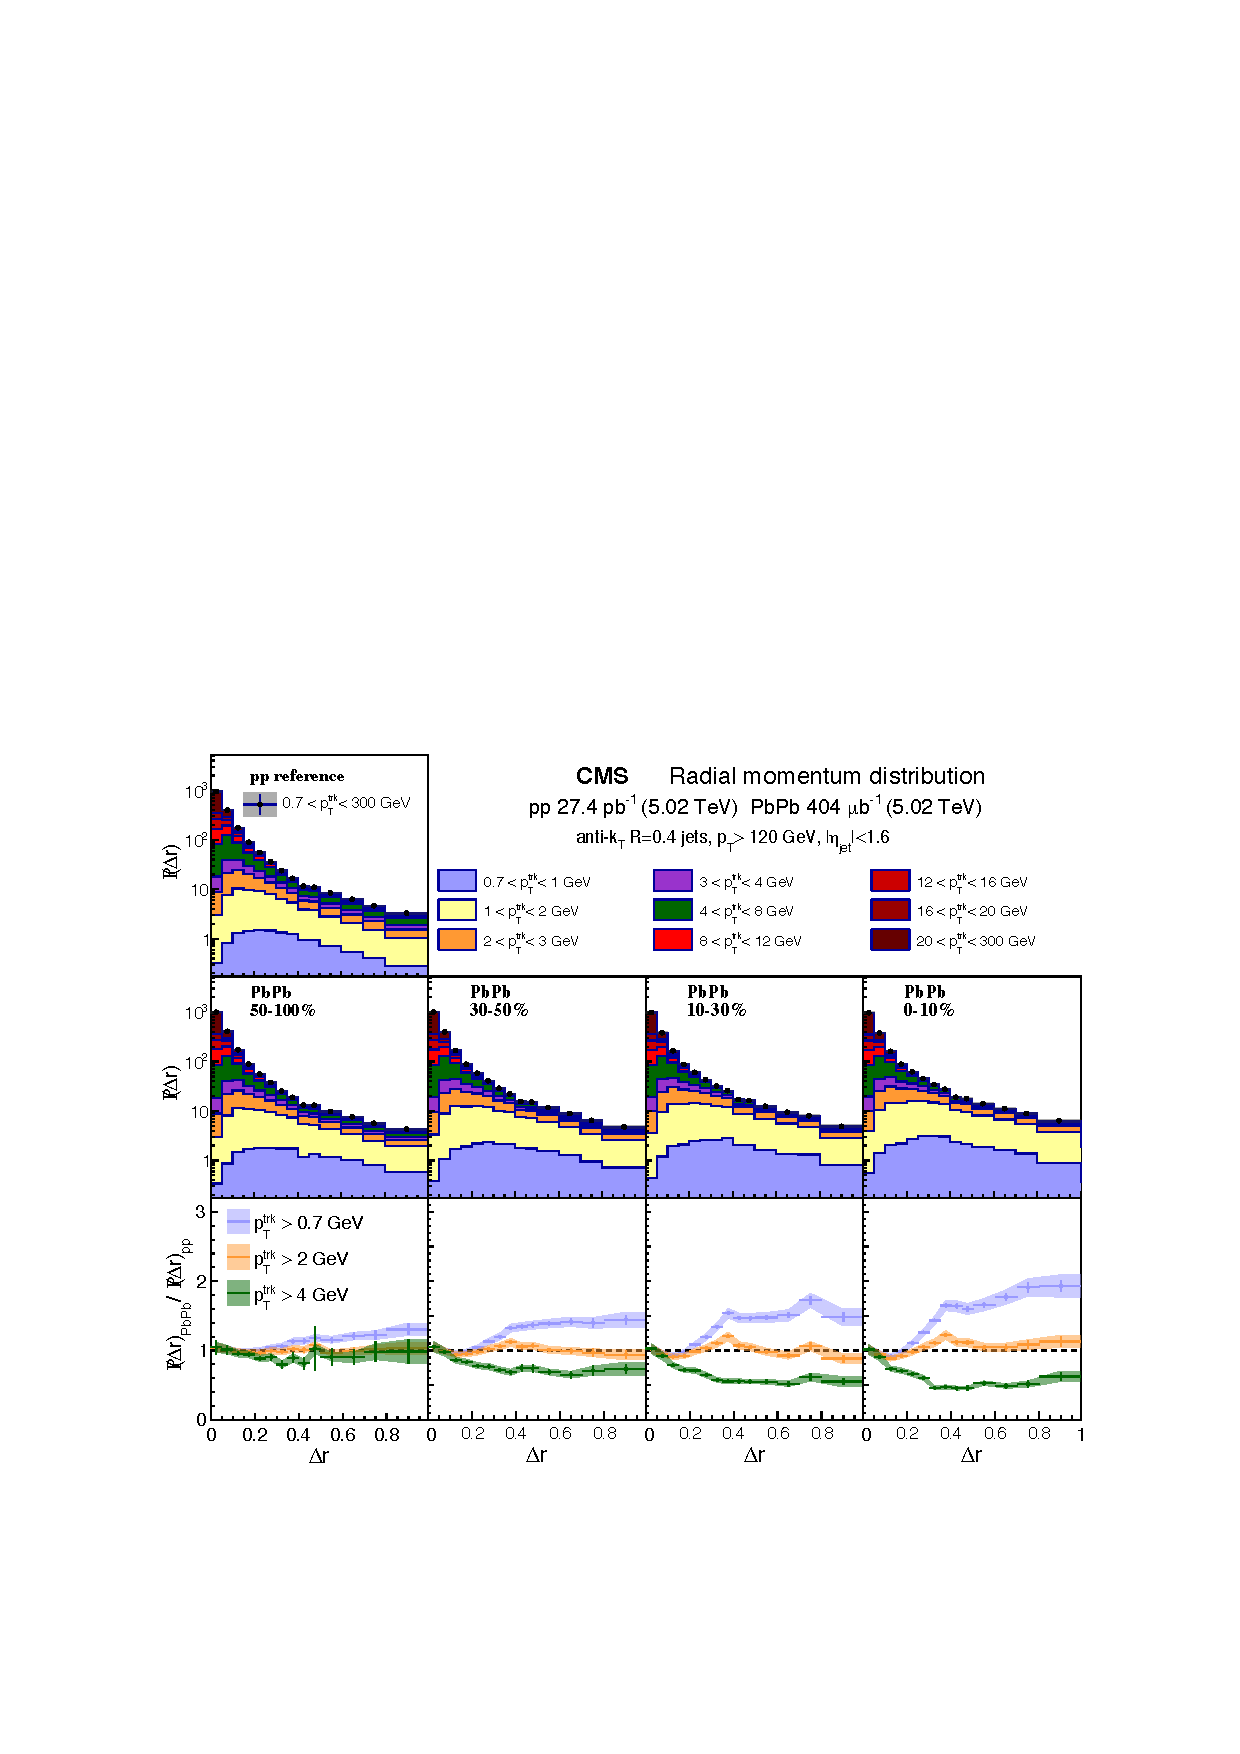
\includegraphics[width=0.75\textwidth]{figures/jetMeasurements/jetshape_cms}
\caption{The jet profile in \pp\ (top) and \pbpb\ (middle) as a function of distance from the jet axis.
The different panels in the middle give the jet shape distribution for different centrality intervals.
The modifications to the jet shape are shown at the bottom, with each panel corresponding to a different centrality.
Figure taken from \cite{Sirunyan:2018jqr}.}
\label{fig:jetshape_cms}
\end{center}
\end{figure}
